

% Titre.
\newcommand{\ulbtitle}{ECON-S101 - Introduction à la microéconomie\\Micael \textsc{Castanheira De Moura}\\Résumé du cours}

% Auteurs: Prénom1 \textsc{Nom1}\\Prénom2 \textsc{Nom2}\\Prénom3 \textsc{Nom3}
\newcommand{\ulbauthors}{Rodrigue \textsc{Van Brande}}

 % Bas de page. Attention, respectez les \_ sinon erreur à la compilation.
\newcommand{\ulbbasdepage}{https://github.com/ULBstudents/ECON-S101-Introduction\_a\_la\_microeconomie-Resume}

% Détails du pdf.
\newcommand{\ulbpdfinfotitle}{ECON-S101 - Introduction à la microéconomie - Résumé du cours}
\newcommand{\ulbpdfinfoauthors}{Rodrigue VAN BRANDE}
\newcommand{\ulbpdfinfolink}{https://github.com/ULBstudents/ECON-S101-Introduction_a_la_microeconomie-Resume}

% Le contenu du pdf.
\newcommand{\ulbpdfinput}{

\section{Séance 2 : l'élasticité}



\subsection{Élasticité de A par rapport à B}
Élasticité d'une variable A par rapport à une autre variable B :
$$\frac{taux\ de\ croissance\ de\ A}{taux\ de\ croissance\ de\ B}=\frac{\Delta A/A}{\Delta B/B}=\frac{dA}{dB}.\frac{B}{A}$$



\subsection{Élasticité-prix de la demande $\eta^d$}
$$\frac{taux\ de\ croissance\ de\ q}{taux\ de\ croissance\ de\ p}=\frac{\Delta q/q}{\Delta p/p}=\frac{dQ}{dp}.\frac{p}{q}$$ 
\begin{flushright}
	(Attention, prendre le Q de la demande.)
\end{flushright}
Donc si P augmente (diminue) de $x\ \%$. $Q^d$ diminue (augmente) de $x.\eta^d\ \%$



\subsection{Élasticité-prix de l'offre $\eta^o$}
$$\frac{taux\ de\ croissance\ de\ q}{taux\ de\ croissance\ de\ p}=\frac{\Delta q/q}{\Delta p/p}=\frac{dQ}{dp}.\frac{p}{q}$$ 
\begin{flushright}
	(Attention, prendre le Q de l'offre.)
\end{flushright}
Donc si P augmente (diminue) de $x\ \%$. $Q^d$ augmente (diminue) de $x.\eta^o\ \%$



\subsection{Élastique, inélastique et élasticité unitaire}
\begin{itemize} 
    \item $\eta > 1$ Offre ou demande élastique ;
    \item $\eta < 1$ Offre ou demande inélastique ;
    \item $\eta = 1$ Offre ou demande élasticité unitaire.
\end{itemize}
En plus...
\begin{itemize}
    \item L’élasticité de la demande vaut 1 quand $Q=\frac{a}{2b}$ ;
    \item Toute droite passant par l’origine a une élasticité constante et unitaire.
\end{itemize}


\subsection{Affirmations vraies}
\begin{tabular}{llll}
	Demande élastique    & P$\nearrow$ un peu,   & Q$\searrow$ beaucoup & RT (P.Q)$\searrow$\\
	Demande élastique    & P$\searrow$ un peu,   & Q$\nearrow$ beaucoup & RT (P.Q)$\nearrow$\\
	Demande inélastique  & P$\nearrow$ beaucoup, & Q$\searrow$ un peu   & RT (P.Q)$\nearrow$\\
	Demande inélastique  & P$\searrow$ beaucoup, & Q$\nearrow$ un peu   & RT (P.Q)$\searrow$
\end{tabular}



\subsection{Parfaitement inélastique et parfaitement élastique}
\begin{center}
    \begin{tabular}{cc}
        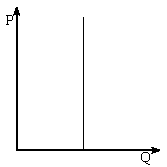
\includegraphics[width=0.25\textwidth]{images/graph_parfaitement_inelastique.pdf}       & 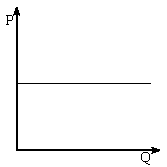
\includegraphics[width=0.25\textwidth]{images/graph_parfaitement_elastique.pdf}\\
        Offre et demande \textcolor[rgb]{1,0,0}{\textit{parfaitement} inélastique} & Offre et demande \textcolor[rgb]{1,0,0}{\textit{parfaitement} élastique}\\
        Élasticité nulle                                                           & Élasticité infinie\\
        $\frac{Q}{P}=\frac{constante}{\infty}=0$                                   &$\frac{Q}{P}=\frac{\infty}{constante}=\infty$
    \end{tabular}
\end{center}



\subsection{Relation entre RT et la demande}



%\begin{tabular}{cp{0.65\textwidth}}
%\begin{minipage}[t]{.3\textwidth}
%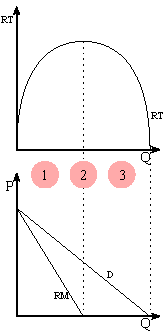
\includegraphics[width=\textwidth]{images/graph_relation_entre_rt_et_demande.pdf}
%\end{minipage}

\begin{minipage}{0.3\textwidth}
    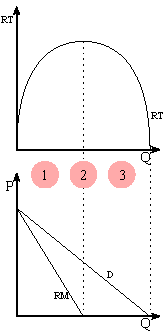
\includegraphics[width=\textwidth]{images/graph_relation_entre_rt_et_demande.pdf}
\end{minipage}
\begin{minipage}{0.6\textwidth}
    Dans la zone 1, la demande est \textcolor[rgb]{1,0,0}{élastique} et la recette marginale est \textcolor[rgb]{1,0,0}{positive}.
		Si les prix diminuent, alors les quantités demandées vont \textcolor[rgb]{1,0,0}{augmenter plus} que proportionnellement et la recette totale va alors \textcolor[rgb]{1,0,0}{augmenter}.
		$$\eta^d > 1$$
		$$RM > 0$$
		$$P \searrow un\ peu\ alors\ Q^d \nearrow beaucoup$$
		$$RT \nearrow$$

		Dans la zone 3, la demande est \textcolor[rgb]{1,0,0}{inélastique} et la recette marginale est \textcolor[rgb]{1,0,0}{négative}.
		Si les prix diminuent, alors les quantités demandées vont \textcolor[rgb]{1,0,0}{augmenter} moins que proportionnellement et la recette totale va alors \textcolor[rgb]{1,0,0}{diminuer}.
		$$\eta^d < 1$$
		$$RM < 0$$
		$$P \searrow beaucoup\ alors\ Q^d \nearrow un\ peu$$
		$$RT \searrow$$

		Au point 2, la demande a une élasticité unitaire tandis que la recette marginale est nulle et la recette totale est maximale.
		$$\eta^d = 1$$
		$$RM = 0$$
		$$RT = max$$
    
    \begin{tabular}{llllll}
        La recette totale:    & $RT$ & $=$ & $PQ$ & $=$ & $aQ - bQ^2$\\
        La recette marginale: & $RM$ & $=$ & $\frac{dRT}{dQ}$ & $=$ & $a - 2bQ$\\
    \end{tabular}
\end{minipage}



\subsection{Taxes et subsides}



\begin{center}
	\begin{tabular}{cc}
	
		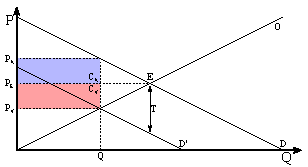
\includegraphics[height=4.5cm]{images/graph_taxe_payee_par_acheteur.pdf} & 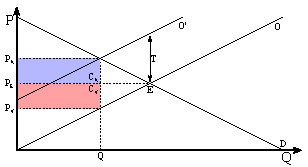
\includegraphics[height=4.5cm]{images/graph_taxe_payee_par_vendeur.pdf}\\
		Taxe payée par l'acheteur                                                & Taxe payée par le vendeur\\
		
		\rule[-0.9cm]{0cm}{0.5cm}\\
		
		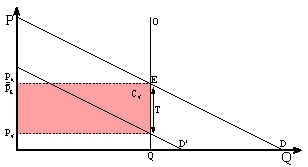
\includegraphics[height=4.5cm]{images/graph_taxe_offre_parfaitement_inelastique.pdf} & 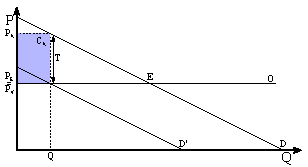
\includegraphics[height=4.5cm]{images/graph_taxe_offre_parfaitement_elastique.pdf}\\
		La taxe sur une offre \textit{parfaitement} inélastique                              & La taxe sur une offre \textit{parfaitement} élastique\\
		La charge est entièrement supportée par le vendeur                                   & La charge est entièrement supportée par l'acheteur\\
		
		\rule[-0.9cm]{0cm}{0.5cm}\\
		
		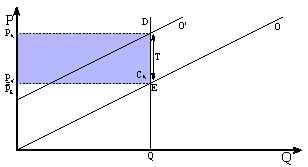
\includegraphics[height=4.5cm]{images/graph_taxe_demande_parfaitement_inelastique.pdf} & 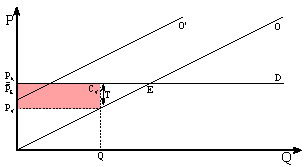
\includegraphics[height=4.5cm]{images/graph_taxe_demande_parfaitement_elastique.pdf}\\
		La taxe sur une demande \textit{parfaitement} inélastique                              & La taxe sur une demande \textit{parfaitement} élastique\\
		La charge est entièrement supportée par l'acheteur                                   & La charge est entièrement supportée par le vendeur\\
	\end{tabular}
\end{center}\newpage
\section{Séance 2 : l'élasticité}



\subsection{Élasticité de A par rapport à B}
Élasticité d'une variable A par rapport à une autre variable B :
$$\frac{taux\ de\ croissance\ de\ A}{taux\ de\ croissance\ de\ B}=\frac{\Delta A/A}{\Delta B/B}=\frac{dA}{dB}.\frac{B}{A}$$



\subsection{Élasticité-prix de la demande $\eta^d$}
$$\frac{taux\ de\ croissance\ de\ q}{taux\ de\ croissance\ de\ p}=\frac{\Delta q/q}{\Delta p/p}=\frac{dQ}{dp}.\frac{p}{q}$$ 
\begin{flushright}
	(Attention, prendre le Q de la demande.)
\end{flushright}
Donc si P augmente (diminue) de $x\ \%$. $Q^d$ diminue (augmente) de $x.\eta^d\ \%$



\subsection{Élasticité-prix de l'offre $\eta^o$}
$$\frac{taux\ de\ croissance\ de\ q}{taux\ de\ croissance\ de\ p}=\frac{\Delta q/q}{\Delta p/p}=\frac{dQ}{dp}.\frac{p}{q}$$ 
\begin{flushright}
	(Attention, prendre le Q de l'offre.)
\end{flushright}
Donc si P augmente (diminue) de $x\ \%$. $Q^d$ augmente (diminue) de $x.\eta^o\ \%$



\subsection{Élastique, inélastique et élasticité unitaire}
\begin{itemize} 
    \item $\eta > 1$ Offre ou demande élastique ;
    \item $\eta < 1$ Offre ou demande inélastique ;
    \item $\eta = 1$ Offre ou demande élasticité unitaire.
\end{itemize}
En plus...
\begin{itemize}
    \item L’élasticité de la demande vaut 1 quand $Q=\frac{a}{2b}$ ;
    \item Toute droite passant par l’origine a une élasticité constante et unitaire.
\end{itemize}


\subsection{Affirmations vraies}
\begin{tabular}{llll}
	Demande élastique    & P$\nearrow$ un peu,   & Q$\searrow$ beaucoup & RT (P.Q)$\searrow$\\
	Demande élastique    & P$\searrow$ un peu,   & Q$\nearrow$ beaucoup & RT (P.Q)$\nearrow$\\
	Demande inélastique  & P$\nearrow$ beaucoup, & Q$\searrow$ un peu   & RT (P.Q)$\nearrow$\\
	Demande inélastique  & P$\searrow$ beaucoup, & Q$\nearrow$ un peu   & RT (P.Q)$\searrow$
\end{tabular}



\subsection{Parfaitement inélastique et parfaitement élastique}
\begin{center}
    \begin{tabular}{cc}
        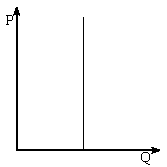
\includegraphics[width=0.25\textwidth]{images/graph_parfaitement_inelastique.pdf}       & 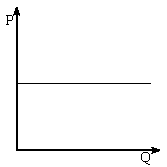
\includegraphics[width=0.25\textwidth]{images/graph_parfaitement_elastique.pdf}\\
        Offre et demande \textcolor[rgb]{1,0,0}{\textit{parfaitement} inélastique} & Offre et demande \textcolor[rgb]{1,0,0}{\textit{parfaitement} élastique}\\
        Élasticité nulle                                                           & Élasticité infinie\\
        $\frac{Q}{P}=\frac{constante}{\infty}=0$                                   &$\frac{Q}{P}=\frac{\infty}{constante}=\infty$
    \end{tabular}
\end{center}



\subsection{Relation entre RT et la demande}



%\begin{tabular}{cp{0.65\textwidth}}
%\begin{minipage}[t]{.3\textwidth}
%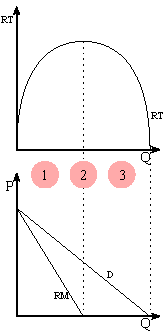
\includegraphics[width=\textwidth]{images/graph_relation_entre_rt_et_demande.pdf}
%\end{minipage}

\begin{minipage}{0.3\textwidth}
    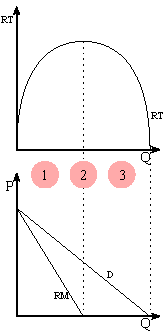
\includegraphics[width=\textwidth]{images/graph_relation_entre_rt_et_demande.pdf}
\end{minipage}
\begin{minipage}{0.6\textwidth}
    Dans la zone 1, la demande est \textcolor[rgb]{1,0,0}{élastique} et la recette marginale est \textcolor[rgb]{1,0,0}{positive}.
		Si les prix diminuent, alors les quantités demandées vont \textcolor[rgb]{1,0,0}{augmenter plus} que proportionnellement et la recette totale va alors \textcolor[rgb]{1,0,0}{augmenter}.
		$$\eta^d > 1$$
		$$RM > 0$$
		$$P \searrow un\ peu\ alors\ Q^d \nearrow beaucoup$$
		$$RT \nearrow$$

		Dans la zone 3, la demande est \textcolor[rgb]{1,0,0}{inélastique} et la recette marginale est \textcolor[rgb]{1,0,0}{négative}.
		Si les prix diminuent, alors les quantités demandées vont \textcolor[rgb]{1,0,0}{augmenter} moins que proportionnellement et la recette totale va alors \textcolor[rgb]{1,0,0}{diminuer}.
		$$\eta^d < 1$$
		$$RM < 0$$
		$$P \searrow beaucoup\ alors\ Q^d \nearrow un\ peu$$
		$$RT \searrow$$

		Au point 2, la demande a une élasticité unitaire tandis que la recette marginale est nulle et la recette totale est maximale.
		$$\eta^d = 1$$
		$$RM = 0$$
		$$RT = max$$
    
    \begin{tabular}{llllll}
        La recette totale:    & $RT$ & $=$ & $PQ$ & $=$ & $aQ - bQ^2$\\
        La recette marginale: & $RM$ & $=$ & $\frac{dRT}{dQ}$ & $=$ & $a - 2bQ$\\
    \end{tabular}
\end{minipage}



\subsection{Taxes et subsides}



\begin{center}
	\begin{tabular}{cc}
	
		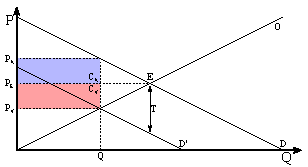
\includegraphics[height=4.5cm]{images/graph_taxe_payee_par_acheteur.pdf} & 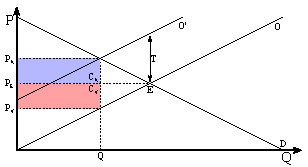
\includegraphics[height=4.5cm]{images/graph_taxe_payee_par_vendeur.pdf}\\
		Taxe payée par l'acheteur                                                & Taxe payée par le vendeur\\
		
		\rule[-0.9cm]{0cm}{0.5cm}\\
		
		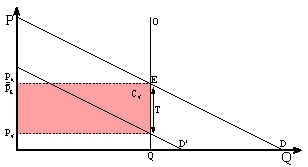
\includegraphics[height=4.5cm]{images/graph_taxe_offre_parfaitement_inelastique.pdf} & 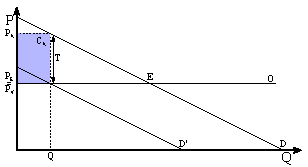
\includegraphics[height=4.5cm]{images/graph_taxe_offre_parfaitement_elastique.pdf}\\
		La taxe sur une offre \textit{parfaitement} inélastique                              & La taxe sur une offre \textit{parfaitement} élastique\\
		La charge est entièrement supportée par le vendeur                                   & La charge est entièrement supportée par l'acheteur\\
		
		\rule[-0.9cm]{0cm}{0.5cm}\\
		
		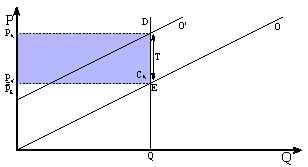
\includegraphics[height=4.5cm]{images/graph_taxe_demande_parfaitement_inelastique.pdf} & 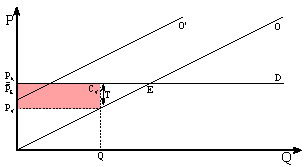
\includegraphics[height=4.5cm]{images/graph_taxe_demande_parfaitement_elastique.pdf}\\
		La taxe sur une demande \textit{parfaitement} inélastique                              & La taxe sur une demande \textit{parfaitement} élastique\\
		La charge est entièrement supportée par l'acheteur                                   & La charge est entièrement supportée par le vendeur\\
	\end{tabular}
\end{center}\newpage
\section{Séance 2 : l'élasticité}



\subsection{Élasticité de A par rapport à B}
Élasticité d'une variable A par rapport à une autre variable B :
$$\frac{taux\ de\ croissance\ de\ A}{taux\ de\ croissance\ de\ B}=\frac{\Delta A/A}{\Delta B/B}=\frac{dA}{dB}.\frac{B}{A}$$



\subsection{Élasticité-prix de la demande $\eta^d$}
$$\frac{taux\ de\ croissance\ de\ q}{taux\ de\ croissance\ de\ p}=\frac{\Delta q/q}{\Delta p/p}=\frac{dQ}{dp}.\frac{p}{q}$$ 
\begin{flushright}
	(Attention, prendre le Q de la demande.)
\end{flushright}
Donc si P augmente (diminue) de $x\ \%$. $Q^d$ diminue (augmente) de $x.\eta^d\ \%$



\subsection{Élasticité-prix de l'offre $\eta^o$}
$$\frac{taux\ de\ croissance\ de\ q}{taux\ de\ croissance\ de\ p}=\frac{\Delta q/q}{\Delta p/p}=\frac{dQ}{dp}.\frac{p}{q}$$ 
\begin{flushright}
	(Attention, prendre le Q de l'offre.)
\end{flushright}
Donc si P augmente (diminue) de $x\ \%$. $Q^d$ augmente (diminue) de $x.\eta^o\ \%$



\subsection{Élastique, inélastique et élasticité unitaire}
\begin{itemize} 
    \item $\eta > 1$ Offre ou demande élastique ;
    \item $\eta < 1$ Offre ou demande inélastique ;
    \item $\eta = 1$ Offre ou demande élasticité unitaire.
\end{itemize}
En plus...
\begin{itemize}
    \item L’élasticité de la demande vaut 1 quand $Q=\frac{a}{2b}$ ;
    \item Toute droite passant par l’origine a une élasticité constante et unitaire.
\end{itemize}


\subsection{Affirmations vraies}
\begin{tabular}{llll}
	Demande élastique    & P$\nearrow$ un peu,   & Q$\searrow$ beaucoup & RT (P.Q)$\searrow$\\
	Demande élastique    & P$\searrow$ un peu,   & Q$\nearrow$ beaucoup & RT (P.Q)$\nearrow$\\
	Demande inélastique  & P$\nearrow$ beaucoup, & Q$\searrow$ un peu   & RT (P.Q)$\nearrow$\\
	Demande inélastique  & P$\searrow$ beaucoup, & Q$\nearrow$ un peu   & RT (P.Q)$\searrow$
\end{tabular}



\subsection{Parfaitement inélastique et parfaitement élastique}
\begin{center}
    \begin{tabular}{cc}
        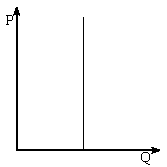
\includegraphics[width=0.25\textwidth]{images/graph_parfaitement_inelastique.pdf}       & 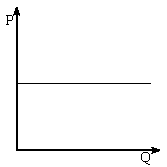
\includegraphics[width=0.25\textwidth]{images/graph_parfaitement_elastique.pdf}\\
        Offre et demande \textcolor[rgb]{1,0,0}{\textit{parfaitement} inélastique} & Offre et demande \textcolor[rgb]{1,0,0}{\textit{parfaitement} élastique}\\
        Élasticité nulle                                                           & Élasticité infinie\\
        $\frac{Q}{P}=\frac{constante}{\infty}=0$                                   &$\frac{Q}{P}=\frac{\infty}{constante}=\infty$
    \end{tabular}
\end{center}



\subsection{Relation entre RT et la demande}



%\begin{tabular}{cp{0.65\textwidth}}
%\begin{minipage}[t]{.3\textwidth}
%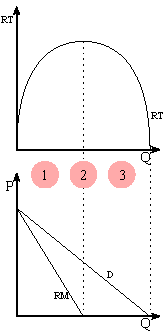
\includegraphics[width=\textwidth]{images/graph_relation_entre_rt_et_demande.pdf}
%\end{minipage}

\begin{minipage}{0.3\textwidth}
    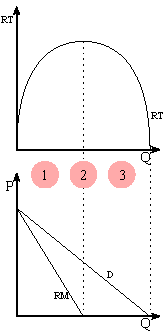
\includegraphics[width=\textwidth]{images/graph_relation_entre_rt_et_demande.pdf}
\end{minipage}
\begin{minipage}{0.6\textwidth}
    Dans la zone 1, la demande est \textcolor[rgb]{1,0,0}{élastique} et la recette marginale est \textcolor[rgb]{1,0,0}{positive}.
		Si les prix diminuent, alors les quantités demandées vont \textcolor[rgb]{1,0,0}{augmenter plus} que proportionnellement et la recette totale va alors \textcolor[rgb]{1,0,0}{augmenter}.
		$$\eta^d > 1$$
		$$RM > 0$$
		$$P \searrow un\ peu\ alors\ Q^d \nearrow beaucoup$$
		$$RT \nearrow$$

		Dans la zone 3, la demande est \textcolor[rgb]{1,0,0}{inélastique} et la recette marginale est \textcolor[rgb]{1,0,0}{négative}.
		Si les prix diminuent, alors les quantités demandées vont \textcolor[rgb]{1,0,0}{augmenter} moins que proportionnellement et la recette totale va alors \textcolor[rgb]{1,0,0}{diminuer}.
		$$\eta^d < 1$$
		$$RM < 0$$
		$$P \searrow beaucoup\ alors\ Q^d \nearrow un\ peu$$
		$$RT \searrow$$

		Au point 2, la demande a une élasticité unitaire tandis que la recette marginale est nulle et la recette totale est maximale.
		$$\eta^d = 1$$
		$$RM = 0$$
		$$RT = max$$
    
    \begin{tabular}{llllll}
        La recette totale:    & $RT$ & $=$ & $PQ$ & $=$ & $aQ - bQ^2$\\
        La recette marginale: & $RM$ & $=$ & $\frac{dRT}{dQ}$ & $=$ & $a - 2bQ$\\
    \end{tabular}
\end{minipage}



\subsection{Taxes et subsides}



\begin{center}
	\begin{tabular}{cc}
	
		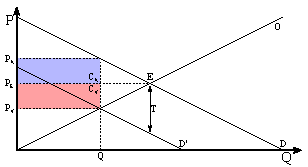
\includegraphics[height=4.5cm]{images/graph_taxe_payee_par_acheteur.pdf} & 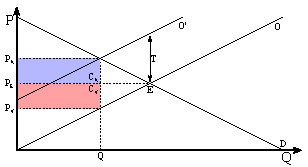
\includegraphics[height=4.5cm]{images/graph_taxe_payee_par_vendeur.pdf}\\
		Taxe payée par l'acheteur                                                & Taxe payée par le vendeur\\
		
		\rule[-0.9cm]{0cm}{0.5cm}\\
		
		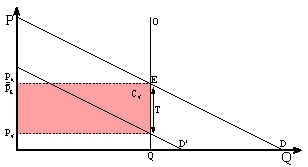
\includegraphics[height=4.5cm]{images/graph_taxe_offre_parfaitement_inelastique.pdf} & 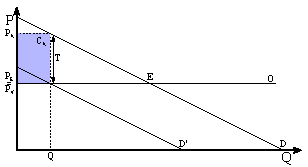
\includegraphics[height=4.5cm]{images/graph_taxe_offre_parfaitement_elastique.pdf}\\
		La taxe sur une offre \textit{parfaitement} inélastique                              & La taxe sur une offre \textit{parfaitement} élastique\\
		La charge est entièrement supportée par le vendeur                                   & La charge est entièrement supportée par l'acheteur\\
		
		\rule[-0.9cm]{0cm}{0.5cm}\\
		
		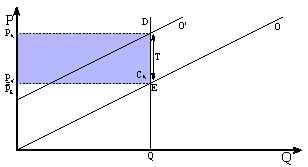
\includegraphics[height=4.5cm]{images/graph_taxe_demande_parfaitement_inelastique.pdf} & 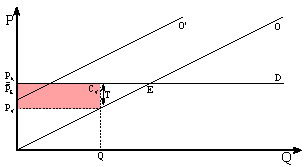
\includegraphics[height=4.5cm]{images/graph_taxe_demande_parfaitement_elastique.pdf}\\
		La taxe sur une demande \textit{parfaitement} inélastique                              & La taxe sur une demande \textit{parfaitement} élastique\\
		La charge est entièrement supportée par l'acheteur                                   & La charge est entièrement supportée par le vendeur\\
	\end{tabular}
\end{center}\newpage
\section{Séance 2 : l'élasticité}



\subsection{Élasticité de A par rapport à B}
Élasticité d'une variable A par rapport à une autre variable B :
$$\frac{taux\ de\ croissance\ de\ A}{taux\ de\ croissance\ de\ B}=\frac{\Delta A/A}{\Delta B/B}=\frac{dA}{dB}.\frac{B}{A}$$



\subsection{Élasticité-prix de la demande $\eta^d$}
$$\frac{taux\ de\ croissance\ de\ q}{taux\ de\ croissance\ de\ p}=\frac{\Delta q/q}{\Delta p/p}=\frac{dQ}{dp}.\frac{p}{q}$$ 
\begin{flushright}
	(Attention, prendre le Q de la demande.)
\end{flushright}
Donc si P augmente (diminue) de $x\ \%$. $Q^d$ diminue (augmente) de $x.\eta^d\ \%$



\subsection{Élasticité-prix de l'offre $\eta^o$}
$$\frac{taux\ de\ croissance\ de\ q}{taux\ de\ croissance\ de\ p}=\frac{\Delta q/q}{\Delta p/p}=\frac{dQ}{dp}.\frac{p}{q}$$ 
\begin{flushright}
	(Attention, prendre le Q de l'offre.)
\end{flushright}
Donc si P augmente (diminue) de $x\ \%$. $Q^d$ augmente (diminue) de $x.\eta^o\ \%$



\subsection{Élastique, inélastique et élasticité unitaire}
\begin{itemize} 
    \item $\eta > 1$ Offre ou demande élastique ;
    \item $\eta < 1$ Offre ou demande inélastique ;
    \item $\eta = 1$ Offre ou demande élasticité unitaire.
\end{itemize}
En plus...
\begin{itemize}
    \item L’élasticité de la demande vaut 1 quand $Q=\frac{a}{2b}$ ;
    \item Toute droite passant par l’origine a une élasticité constante et unitaire.
\end{itemize}


\subsection{Affirmations vraies}
\begin{tabular}{llll}
	Demande élastique    & P$\nearrow$ un peu,   & Q$\searrow$ beaucoup & RT (P.Q)$\searrow$\\
	Demande élastique    & P$\searrow$ un peu,   & Q$\nearrow$ beaucoup & RT (P.Q)$\nearrow$\\
	Demande inélastique  & P$\nearrow$ beaucoup, & Q$\searrow$ un peu   & RT (P.Q)$\nearrow$\\
	Demande inélastique  & P$\searrow$ beaucoup, & Q$\nearrow$ un peu   & RT (P.Q)$\searrow$
\end{tabular}



\subsection{Parfaitement inélastique et parfaitement élastique}
\begin{center}
    \begin{tabular}{cc}
        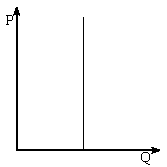
\includegraphics[width=0.25\textwidth]{images/graph_parfaitement_inelastique.pdf}       & 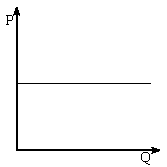
\includegraphics[width=0.25\textwidth]{images/graph_parfaitement_elastique.pdf}\\
        Offre et demande \textcolor[rgb]{1,0,0}{\textit{parfaitement} inélastique} & Offre et demande \textcolor[rgb]{1,0,0}{\textit{parfaitement} élastique}\\
        Élasticité nulle                                                           & Élasticité infinie\\
        $\frac{Q}{P}=\frac{constante}{\infty}=0$                                   &$\frac{Q}{P}=\frac{\infty}{constante}=\infty$
    \end{tabular}
\end{center}



\subsection{Relation entre RT et la demande}



%\begin{tabular}{cp{0.65\textwidth}}
%\begin{minipage}[t]{.3\textwidth}
%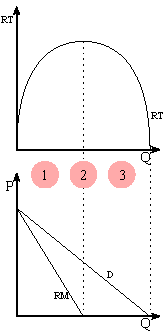
\includegraphics[width=\textwidth]{images/graph_relation_entre_rt_et_demande.pdf}
%\end{minipage}

\begin{minipage}{0.3\textwidth}
    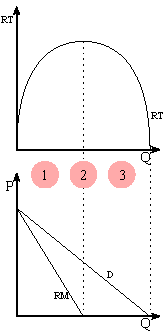
\includegraphics[width=\textwidth]{images/graph_relation_entre_rt_et_demande.pdf}
\end{minipage}
\begin{minipage}{0.6\textwidth}
    Dans la zone 1, la demande est \textcolor[rgb]{1,0,0}{élastique} et la recette marginale est \textcolor[rgb]{1,0,0}{positive}.
		Si les prix diminuent, alors les quantités demandées vont \textcolor[rgb]{1,0,0}{augmenter plus} que proportionnellement et la recette totale va alors \textcolor[rgb]{1,0,0}{augmenter}.
		$$\eta^d > 1$$
		$$RM > 0$$
		$$P \searrow un\ peu\ alors\ Q^d \nearrow beaucoup$$
		$$RT \nearrow$$

		Dans la zone 3, la demande est \textcolor[rgb]{1,0,0}{inélastique} et la recette marginale est \textcolor[rgb]{1,0,0}{négative}.
		Si les prix diminuent, alors les quantités demandées vont \textcolor[rgb]{1,0,0}{augmenter} moins que proportionnellement et la recette totale va alors \textcolor[rgb]{1,0,0}{diminuer}.
		$$\eta^d < 1$$
		$$RM < 0$$
		$$P \searrow beaucoup\ alors\ Q^d \nearrow un\ peu$$
		$$RT \searrow$$

		Au point 2, la demande a une élasticité unitaire tandis que la recette marginale est nulle et la recette totale est maximale.
		$$\eta^d = 1$$
		$$RM = 0$$
		$$RT = max$$
    
    \begin{tabular}{llllll}
        La recette totale:    & $RT$ & $=$ & $PQ$ & $=$ & $aQ - bQ^2$\\
        La recette marginale: & $RM$ & $=$ & $\frac{dRT}{dQ}$ & $=$ & $a - 2bQ$\\
    \end{tabular}
\end{minipage}



\subsection{Taxes et subsides}



\begin{center}
	\begin{tabular}{cc}
	
		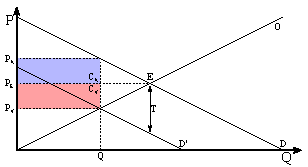
\includegraphics[height=4.5cm]{images/graph_taxe_payee_par_acheteur.pdf} & 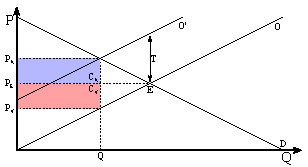
\includegraphics[height=4.5cm]{images/graph_taxe_payee_par_vendeur.pdf}\\
		Taxe payée par l'acheteur                                                & Taxe payée par le vendeur\\
		
		\rule[-0.9cm]{0cm}{0.5cm}\\
		
		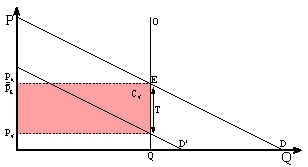
\includegraphics[height=4.5cm]{images/graph_taxe_offre_parfaitement_inelastique.pdf} & 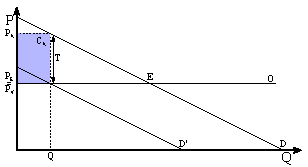
\includegraphics[height=4.5cm]{images/graph_taxe_offre_parfaitement_elastique.pdf}\\
		La taxe sur une offre \textit{parfaitement} inélastique                              & La taxe sur une offre \textit{parfaitement} élastique\\
		La charge est entièrement supportée par le vendeur                                   & La charge est entièrement supportée par l'acheteur\\
		
		\rule[-0.9cm]{0cm}{0.5cm}\\
		
		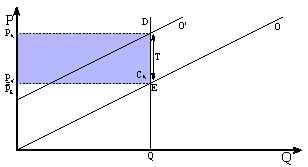
\includegraphics[height=4.5cm]{images/graph_taxe_demande_parfaitement_inelastique.pdf} & 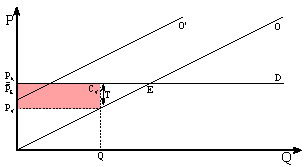
\includegraphics[height=4.5cm]{images/graph_taxe_demande_parfaitement_elastique.pdf}\\
		La taxe sur une demande \textit{parfaitement} inélastique                              & La taxe sur une demande \textit{parfaitement} élastique\\
		La charge est entièrement supportée par l'acheteur                                   & La charge est entièrement supportée par le vendeur\\
	\end{tabular}
\end{center}\newpage
\section{Séance 2 : l'élasticité}



\subsection{Élasticité de A par rapport à B}
Élasticité d'une variable A par rapport à une autre variable B :
$$\frac{taux\ de\ croissance\ de\ A}{taux\ de\ croissance\ de\ B}=\frac{\Delta A/A}{\Delta B/B}=\frac{dA}{dB}.\frac{B}{A}$$



\subsection{Élasticité-prix de la demande $\eta^d$}
$$\frac{taux\ de\ croissance\ de\ q}{taux\ de\ croissance\ de\ p}=\frac{\Delta q/q}{\Delta p/p}=\frac{dQ}{dp}.\frac{p}{q}$$ 
\begin{flushright}
	(Attention, prendre le Q de la demande.)
\end{flushright}
Donc si P augmente (diminue) de $x\ \%$. $Q^d$ diminue (augmente) de $x.\eta^d\ \%$



\subsection{Élasticité-prix de l'offre $\eta^o$}
$$\frac{taux\ de\ croissance\ de\ q}{taux\ de\ croissance\ de\ p}=\frac{\Delta q/q}{\Delta p/p}=\frac{dQ}{dp}.\frac{p}{q}$$ 
\begin{flushright}
	(Attention, prendre le Q de l'offre.)
\end{flushright}
Donc si P augmente (diminue) de $x\ \%$. $Q^d$ augmente (diminue) de $x.\eta^o\ \%$



\subsection{Élastique, inélastique et élasticité unitaire}
\begin{itemize} 
    \item $\eta > 1$ Offre ou demande élastique ;
    \item $\eta < 1$ Offre ou demande inélastique ;
    \item $\eta = 1$ Offre ou demande élasticité unitaire.
\end{itemize}
En plus...
\begin{itemize}
    \item L’élasticité de la demande vaut 1 quand $Q=\frac{a}{2b}$ ;
    \item Toute droite passant par l’origine a une élasticité constante et unitaire.
\end{itemize}


\subsection{Affirmations vraies}
\begin{tabular}{llll}
	Demande élastique    & P$\nearrow$ un peu,   & Q$\searrow$ beaucoup & RT (P.Q)$\searrow$\\
	Demande élastique    & P$\searrow$ un peu,   & Q$\nearrow$ beaucoup & RT (P.Q)$\nearrow$\\
	Demande inélastique  & P$\nearrow$ beaucoup, & Q$\searrow$ un peu   & RT (P.Q)$\nearrow$\\
	Demande inélastique  & P$\searrow$ beaucoup, & Q$\nearrow$ un peu   & RT (P.Q)$\searrow$
\end{tabular}



\subsection{Parfaitement inélastique et parfaitement élastique}
\begin{center}
    \begin{tabular}{cc}
        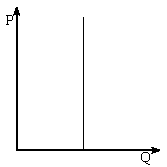
\includegraphics[width=0.25\textwidth]{images/graph_parfaitement_inelastique.pdf}       & 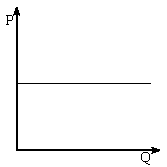
\includegraphics[width=0.25\textwidth]{images/graph_parfaitement_elastique.pdf}\\
        Offre et demande \textcolor[rgb]{1,0,0}{\textit{parfaitement} inélastique} & Offre et demande \textcolor[rgb]{1,0,0}{\textit{parfaitement} élastique}\\
        Élasticité nulle                                                           & Élasticité infinie\\
        $\frac{Q}{P}=\frac{constante}{\infty}=0$                                   &$\frac{Q}{P}=\frac{\infty}{constante}=\infty$
    \end{tabular}
\end{center}



\subsection{Relation entre RT et la demande}



%\begin{tabular}{cp{0.65\textwidth}}
%\begin{minipage}[t]{.3\textwidth}
%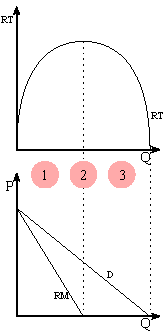
\includegraphics[width=\textwidth]{images/graph_relation_entre_rt_et_demande.pdf}
%\end{minipage}

\begin{minipage}{0.3\textwidth}
    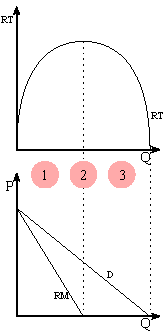
\includegraphics[width=\textwidth]{images/graph_relation_entre_rt_et_demande.pdf}
\end{minipage}
\begin{minipage}{0.6\textwidth}
    Dans la zone 1, la demande est \textcolor[rgb]{1,0,0}{élastique} et la recette marginale est \textcolor[rgb]{1,0,0}{positive}.
		Si les prix diminuent, alors les quantités demandées vont \textcolor[rgb]{1,0,0}{augmenter plus} que proportionnellement et la recette totale va alors \textcolor[rgb]{1,0,0}{augmenter}.
		$$\eta^d > 1$$
		$$RM > 0$$
		$$P \searrow un\ peu\ alors\ Q^d \nearrow beaucoup$$
		$$RT \nearrow$$

		Dans la zone 3, la demande est \textcolor[rgb]{1,0,0}{inélastique} et la recette marginale est \textcolor[rgb]{1,0,0}{négative}.
		Si les prix diminuent, alors les quantités demandées vont \textcolor[rgb]{1,0,0}{augmenter} moins que proportionnellement et la recette totale va alors \textcolor[rgb]{1,0,0}{diminuer}.
		$$\eta^d < 1$$
		$$RM < 0$$
		$$P \searrow beaucoup\ alors\ Q^d \nearrow un\ peu$$
		$$RT \searrow$$

		Au point 2, la demande a une élasticité unitaire tandis que la recette marginale est nulle et la recette totale est maximale.
		$$\eta^d = 1$$
		$$RM = 0$$
		$$RT = max$$
    
    \begin{tabular}{llllll}
        La recette totale:    & $RT$ & $=$ & $PQ$ & $=$ & $aQ - bQ^2$\\
        La recette marginale: & $RM$ & $=$ & $\frac{dRT}{dQ}$ & $=$ & $a - 2bQ$\\
    \end{tabular}
\end{minipage}



\subsection{Taxes et subsides}



\begin{center}
	\begin{tabular}{cc}
	
		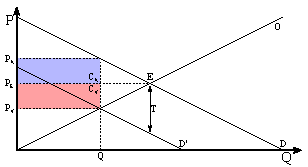
\includegraphics[height=4.5cm]{images/graph_taxe_payee_par_acheteur.pdf} & 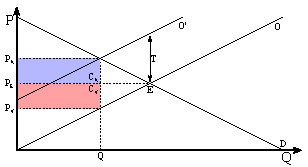
\includegraphics[height=4.5cm]{images/graph_taxe_payee_par_vendeur.pdf}\\
		Taxe payée par l'acheteur                                                & Taxe payée par le vendeur\\
		
		\rule[-0.9cm]{0cm}{0.5cm}\\
		
		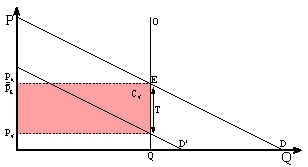
\includegraphics[height=4.5cm]{images/graph_taxe_offre_parfaitement_inelastique.pdf} & 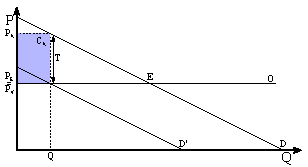
\includegraphics[height=4.5cm]{images/graph_taxe_offre_parfaitement_elastique.pdf}\\
		La taxe sur une offre \textit{parfaitement} inélastique                              & La taxe sur une offre \textit{parfaitement} élastique\\
		La charge est entièrement supportée par le vendeur                                   & La charge est entièrement supportée par l'acheteur\\
		
		\rule[-0.9cm]{0cm}{0.5cm}\\
		
		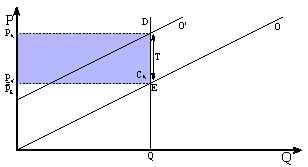
\includegraphics[height=4.5cm]{images/graph_taxe_demande_parfaitement_inelastique.pdf} & 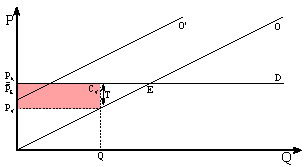
\includegraphics[height=4.5cm]{images/graph_taxe_demande_parfaitement_elastique.pdf}\\
		La taxe sur une demande \textit{parfaitement} inélastique                              & La taxe sur une demande \textit{parfaitement} élastique\\
		La charge est entièrement supportée par l'acheteur                                   & La charge est entièrement supportée par le vendeur\\
	\end{tabular}
\end{center}\newpage
\section{Séance 2 : l'élasticité}



\subsection{Élasticité de A par rapport à B}
Élasticité d'une variable A par rapport à une autre variable B :
$$\frac{taux\ de\ croissance\ de\ A}{taux\ de\ croissance\ de\ B}=\frac{\Delta A/A}{\Delta B/B}=\frac{dA}{dB}.\frac{B}{A}$$



\subsection{Élasticité-prix de la demande $\eta^d$}
$$\frac{taux\ de\ croissance\ de\ q}{taux\ de\ croissance\ de\ p}=\frac{\Delta q/q}{\Delta p/p}=\frac{dQ}{dp}.\frac{p}{q}$$ 
\begin{flushright}
	(Attention, prendre le Q de la demande.)
\end{flushright}
Donc si P augmente (diminue) de $x\ \%$. $Q^d$ diminue (augmente) de $x.\eta^d\ \%$



\subsection{Élasticité-prix de l'offre $\eta^o$}
$$\frac{taux\ de\ croissance\ de\ q}{taux\ de\ croissance\ de\ p}=\frac{\Delta q/q}{\Delta p/p}=\frac{dQ}{dp}.\frac{p}{q}$$ 
\begin{flushright}
	(Attention, prendre le Q de l'offre.)
\end{flushright}
Donc si P augmente (diminue) de $x\ \%$. $Q^d$ augmente (diminue) de $x.\eta^o\ \%$



\subsection{Élastique, inélastique et élasticité unitaire}
\begin{itemize} 
    \item $\eta > 1$ Offre ou demande élastique ;
    \item $\eta < 1$ Offre ou demande inélastique ;
    \item $\eta = 1$ Offre ou demande élasticité unitaire.
\end{itemize}
En plus...
\begin{itemize}
    \item L’élasticité de la demande vaut 1 quand $Q=\frac{a}{2b}$ ;
    \item Toute droite passant par l’origine a une élasticité constante et unitaire.
\end{itemize}


\subsection{Affirmations vraies}
\begin{tabular}{llll}
	Demande élastique    & P$\nearrow$ un peu,   & Q$\searrow$ beaucoup & RT (P.Q)$\searrow$\\
	Demande élastique    & P$\searrow$ un peu,   & Q$\nearrow$ beaucoup & RT (P.Q)$\nearrow$\\
	Demande inélastique  & P$\nearrow$ beaucoup, & Q$\searrow$ un peu   & RT (P.Q)$\nearrow$\\
	Demande inélastique  & P$\searrow$ beaucoup, & Q$\nearrow$ un peu   & RT (P.Q)$\searrow$
\end{tabular}



\subsection{Parfaitement inélastique et parfaitement élastique}
\begin{center}
    \begin{tabular}{cc}
        \includegraphics[width=0.25\textwidth]{images/graph_parfaitement_inelastique.pdf}       & \includegraphics[width=0.25\textwidth]{images/graph_parfaitement_elastique.pdf}\\
        Offre et demande \textcolor[rgb]{1,0,0}{\textit{parfaitement} inélastique} & Offre et demande \textcolor[rgb]{1,0,0}{\textit{parfaitement} élastique}\\
        Élasticité nulle                                                           & Élasticité infinie\\
        $\frac{Q}{P}=\frac{constante}{\infty}=0$                                   &$\frac{Q}{P}=\frac{\infty}{constante}=\infty$
    \end{tabular}
\end{center}



\subsection{Relation entre RT et la demande}



%\begin{tabular}{cp{0.65\textwidth}}
%\begin{minipage}[t]{.3\textwidth}
%\includegraphics[width=\textwidth]{images/graph_relation_entre_rt_et_demande.pdf}
%\end{minipage}

\begin{minipage}{0.3\textwidth}
    \includegraphics[width=\textwidth]{images/graph_relation_entre_rt_et_demande.pdf}
\end{minipage}
\begin{minipage}{0.6\textwidth}
    Dans la zone 1, la demande est \textcolor[rgb]{1,0,0}{élastique} et la recette marginale est \textcolor[rgb]{1,0,0}{positive}.
		Si les prix diminuent, alors les quantités demandées vont \textcolor[rgb]{1,0,0}{augmenter plus} que proportionnellement et la recette totale va alors \textcolor[rgb]{1,0,0}{augmenter}.
		$$\eta^d > 1$$
		$$RM > 0$$
		$$P \searrow un\ peu\ alors\ Q^d \nearrow beaucoup$$
		$$RT \nearrow$$

		Dans la zone 3, la demande est \textcolor[rgb]{1,0,0}{inélastique} et la recette marginale est \textcolor[rgb]{1,0,0}{négative}.
		Si les prix diminuent, alors les quantités demandées vont \textcolor[rgb]{1,0,0}{augmenter} moins que proportionnellement et la recette totale va alors \textcolor[rgb]{1,0,0}{diminuer}.
		$$\eta^d < 1$$
		$$RM < 0$$
		$$P \searrow beaucoup\ alors\ Q^d \nearrow un\ peu$$
		$$RT \searrow$$

		Au point 2, la demande a une élasticité unitaire tandis que la recette marginale est nulle et la recette totale est maximale.
		$$\eta^d = 1$$
		$$RM = 0$$
		$$RT = max$$
    
    \begin{tabular}{llllll}
        La recette totale:    & $RT$ & $=$ & $PQ$ & $=$ & $aQ - bQ^2$\\
        La recette marginale: & $RM$ & $=$ & $\frac{dRT}{dQ}$ & $=$ & $a - 2bQ$\\
    \end{tabular}
\end{minipage}



\subsection{Taxes et subsides}



\begin{center}
	\begin{tabular}{cc}
	
		\includegraphics[height=4.5cm]{images/graph_taxe_payee_par_acheteur.pdf} & \includegraphics[height=4.5cm]{images/graph_taxe_payee_par_vendeur.pdf}\\
		Taxe payée par l'acheteur                                                & Taxe payée par le vendeur\\
		
		\rule[-0.9cm]{0cm}{0.5cm}\\
		
		\includegraphics[height=4.5cm]{images/graph_taxe_offre_parfaitement_inelastique.pdf} & \includegraphics[height=4.5cm]{images/graph_taxe_offre_parfaitement_elastique.pdf}\\
		La taxe sur une offre \textit{parfaitement} inélastique                              & La taxe sur une offre \textit{parfaitement} élastique\\
		La charge est entièrement supportée par le vendeur                                   & La charge est entièrement supportée par l'acheteur\\
		
		\rule[-0.9cm]{0cm}{0.5cm}\\
		
		\includegraphics[height=4.5cm]{images/graph_taxe_demande_parfaitement_inelastique.pdf} & \includegraphics[height=4.5cm]{images/graph_taxe_demande_parfaitement_elastique.pdf}\\
		La taxe sur une demande \textit{parfaitement} inélastique                              & La taxe sur une demande \textit{parfaitement} élastique\\
		La charge est entièrement supportée par l'acheteur                                   & La charge est entièrement supportée par le vendeur\\
	\end{tabular}
\end{center}\newpage
\section{Séance 2 : l'élasticité}



\subsection{Élasticité de A par rapport à B}
Élasticité d'une variable A par rapport à une autre variable B :
$$\frac{taux\ de\ croissance\ de\ A}{taux\ de\ croissance\ de\ B}=\frac{\Delta A/A}{\Delta B/B}=\frac{dA}{dB}.\frac{B}{A}$$



\subsection{Élasticité-prix de la demande $\eta^d$}
$$\frac{taux\ de\ croissance\ de\ q}{taux\ de\ croissance\ de\ p}=\frac{\Delta q/q}{\Delta p/p}=\frac{dQ}{dp}.\frac{p}{q}$$ 
\begin{flushright}
	(Attention, prendre le Q de la demande.)
\end{flushright}
Donc si P augmente (diminue) de $x\ \%$. $Q^d$ diminue (augmente) de $x.\eta^d\ \%$



\subsection{Élasticité-prix de l'offre $\eta^o$}
$$\frac{taux\ de\ croissance\ de\ q}{taux\ de\ croissance\ de\ p}=\frac{\Delta q/q}{\Delta p/p}=\frac{dQ}{dp}.\frac{p}{q}$$ 
\begin{flushright}
	(Attention, prendre le Q de l'offre.)
\end{flushright}
Donc si P augmente (diminue) de $x\ \%$. $Q^d$ augmente (diminue) de $x.\eta^o\ \%$



\subsection{Élastique, inélastique et élasticité unitaire}
\begin{itemize} 
    \item $\eta > 1$ Offre ou demande élastique ;
    \item $\eta < 1$ Offre ou demande inélastique ;
    \item $\eta = 1$ Offre ou demande élasticité unitaire.
\end{itemize}
En plus...
\begin{itemize}
    \item L’élasticité de la demande vaut 1 quand $Q=\frac{a}{2b}$ ;
    \item Toute droite passant par l’origine a une élasticité constante et unitaire.
\end{itemize}


\subsection{Affirmations vraies}
\begin{tabular}{llll}
	Demande élastique    & P$\nearrow$ un peu,   & Q$\searrow$ beaucoup & RT (P.Q)$\searrow$\\
	Demande élastique    & P$\searrow$ un peu,   & Q$\nearrow$ beaucoup & RT (P.Q)$\nearrow$\\
	Demande inélastique  & P$\nearrow$ beaucoup, & Q$\searrow$ un peu   & RT (P.Q)$\nearrow$\\
	Demande inélastique  & P$\searrow$ beaucoup, & Q$\nearrow$ un peu   & RT (P.Q)$\searrow$
\end{tabular}



\subsection{Parfaitement inélastique et parfaitement élastique}
\begin{center}
    \begin{tabular}{cc}
        \includegraphics[width=0.25\textwidth]{images/graph_parfaitement_inelastique.pdf}       & \includegraphics[width=0.25\textwidth]{images/graph_parfaitement_elastique.pdf}\\
        Offre et demande \textcolor[rgb]{1,0,0}{\textit{parfaitement} inélastique} & Offre et demande \textcolor[rgb]{1,0,0}{\textit{parfaitement} élastique}\\
        Élasticité nulle                                                           & Élasticité infinie\\
        $\frac{Q}{P}=\frac{constante}{\infty}=0$                                   &$\frac{Q}{P}=\frac{\infty}{constante}=\infty$
    \end{tabular}
\end{center}



\subsection{Relation entre RT et la demande}



%\begin{tabular}{cp{0.65\textwidth}}
%\begin{minipage}[t]{.3\textwidth}
%\includegraphics[width=\textwidth]{images/graph_relation_entre_rt_et_demande.pdf}
%\end{minipage}

\begin{minipage}{0.3\textwidth}
    \includegraphics[width=\textwidth]{images/graph_relation_entre_rt_et_demande.pdf}
\end{minipage}
\begin{minipage}{0.6\textwidth}
    Dans la zone 1, la demande est \textcolor[rgb]{1,0,0}{élastique} et la recette marginale est \textcolor[rgb]{1,0,0}{positive}.
		Si les prix diminuent, alors les quantités demandées vont \textcolor[rgb]{1,0,0}{augmenter plus} que proportionnellement et la recette totale va alors \textcolor[rgb]{1,0,0}{augmenter}.
		$$\eta^d > 1$$
		$$RM > 0$$
		$$P \searrow un\ peu\ alors\ Q^d \nearrow beaucoup$$
		$$RT \nearrow$$

		Dans la zone 3, la demande est \textcolor[rgb]{1,0,0}{inélastique} et la recette marginale est \textcolor[rgb]{1,0,0}{négative}.
		Si les prix diminuent, alors les quantités demandées vont \textcolor[rgb]{1,0,0}{augmenter} moins que proportionnellement et la recette totale va alors \textcolor[rgb]{1,0,0}{diminuer}.
		$$\eta^d < 1$$
		$$RM < 0$$
		$$P \searrow beaucoup\ alors\ Q^d \nearrow un\ peu$$
		$$RT \searrow$$

		Au point 2, la demande a une élasticité unitaire tandis que la recette marginale est nulle et la recette totale est maximale.
		$$\eta^d = 1$$
		$$RM = 0$$
		$$RT = max$$
    
    \begin{tabular}{llllll}
        La recette totale:    & $RT$ & $=$ & $PQ$ & $=$ & $aQ - bQ^2$\\
        La recette marginale: & $RM$ & $=$ & $\frac{dRT}{dQ}$ & $=$ & $a - 2bQ$\\
    \end{tabular}
\end{minipage}



\subsection{Taxes et subsides}



\begin{center}
	\begin{tabular}{cc}
	
		\includegraphics[height=4.5cm]{images/graph_taxe_payee_par_acheteur.pdf} & \includegraphics[height=4.5cm]{images/graph_taxe_payee_par_vendeur.pdf}\\
		Taxe payée par l'acheteur                                                & Taxe payée par le vendeur\\
		
		\rule[-0.9cm]{0cm}{0.5cm}\\
		
		\includegraphics[height=4.5cm]{images/graph_taxe_offre_parfaitement_inelastique.pdf} & \includegraphics[height=4.5cm]{images/graph_taxe_offre_parfaitement_elastique.pdf}\\
		La taxe sur une offre \textit{parfaitement} inélastique                              & La taxe sur une offre \textit{parfaitement} élastique\\
		La charge est entièrement supportée par le vendeur                                   & La charge est entièrement supportée par l'acheteur\\
		
		\rule[-0.9cm]{0cm}{0.5cm}\\
		
		\includegraphics[height=4.5cm]{images/graph_taxe_demande_parfaitement_inelastique.pdf} & \includegraphics[height=4.5cm]{images/graph_taxe_demande_parfaitement_elastique.pdf}\\
		La taxe sur une demande \textit{parfaitement} inélastique                              & La taxe sur une demande \textit{parfaitement} élastique\\
		La charge est entièrement supportée par l'acheteur                                   & La charge est entièrement supportée par le vendeur\\
	\end{tabular}
\end{center}\newpage
\section{Séance 2 : l'élasticité}



\subsection{Élasticité de A par rapport à B}
Élasticité d'une variable A par rapport à une autre variable B :
$$\frac{taux\ de\ croissance\ de\ A}{taux\ de\ croissance\ de\ B}=\frac{\Delta A/A}{\Delta B/B}=\frac{dA}{dB}.\frac{B}{A}$$



\subsection{Élasticité-prix de la demande $\eta^d$}
$$\frac{taux\ de\ croissance\ de\ q}{taux\ de\ croissance\ de\ p}=\frac{\Delta q/q}{\Delta p/p}=\frac{dQ}{dp}.\frac{p}{q}$$ 
\begin{flushright}
	(Attention, prendre le Q de la demande.)
\end{flushright}
Donc si P augmente (diminue) de $x\ \%$. $Q^d$ diminue (augmente) de $x.\eta^d\ \%$



\subsection{Élasticité-prix de l'offre $\eta^o$}
$$\frac{taux\ de\ croissance\ de\ q}{taux\ de\ croissance\ de\ p}=\frac{\Delta q/q}{\Delta p/p}=\frac{dQ}{dp}.\frac{p}{q}$$ 
\begin{flushright}
	(Attention, prendre le Q de l'offre.)
\end{flushright}
Donc si P augmente (diminue) de $x\ \%$. $Q^d$ augmente (diminue) de $x.\eta^o\ \%$



\subsection{Élastique, inélastique et élasticité unitaire}
\begin{itemize} 
    \item $\eta > 1$ Offre ou demande élastique ;
    \item $\eta < 1$ Offre ou demande inélastique ;
    \item $\eta = 1$ Offre ou demande élasticité unitaire.
\end{itemize}
En plus...
\begin{itemize}
    \item L’élasticité de la demande vaut 1 quand $Q=\frac{a}{2b}$ ;
    \item Toute droite passant par l’origine a une élasticité constante et unitaire.
\end{itemize}


\subsection{Affirmations vraies}
\begin{tabular}{llll}
	Demande élastique    & P$\nearrow$ un peu,   & Q$\searrow$ beaucoup & RT (P.Q)$\searrow$\\
	Demande élastique    & P$\searrow$ un peu,   & Q$\nearrow$ beaucoup & RT (P.Q)$\nearrow$\\
	Demande inélastique  & P$\nearrow$ beaucoup, & Q$\searrow$ un peu   & RT (P.Q)$\nearrow$\\
	Demande inélastique  & P$\searrow$ beaucoup, & Q$\nearrow$ un peu   & RT (P.Q)$\searrow$
\end{tabular}



\subsection{Parfaitement inélastique et parfaitement élastique}
\begin{center}
    \begin{tabular}{cc}
        \includegraphics[width=0.25\textwidth]{images/graph_parfaitement_inelastique.pdf}       & \includegraphics[width=0.25\textwidth]{images/graph_parfaitement_elastique.pdf}\\
        Offre et demande \textcolor[rgb]{1,0,0}{\textit{parfaitement} inélastique} & Offre et demande \textcolor[rgb]{1,0,0}{\textit{parfaitement} élastique}\\
        Élasticité nulle                                                           & Élasticité infinie\\
        $\frac{Q}{P}=\frac{constante}{\infty}=0$                                   &$\frac{Q}{P}=\frac{\infty}{constante}=\infty$
    \end{tabular}
\end{center}



\subsection{Relation entre RT et la demande}



%\begin{tabular}{cp{0.65\textwidth}}
%\begin{minipage}[t]{.3\textwidth}
%\includegraphics[width=\textwidth]{images/graph_relation_entre_rt_et_demande.pdf}
%\end{minipage}

\begin{minipage}{0.3\textwidth}
    \includegraphics[width=\textwidth]{images/graph_relation_entre_rt_et_demande.pdf}
\end{minipage}
\begin{minipage}{0.6\textwidth}
    Dans la zone 1, la demande est \textcolor[rgb]{1,0,0}{élastique} et la recette marginale est \textcolor[rgb]{1,0,0}{positive}.
		Si les prix diminuent, alors les quantités demandées vont \textcolor[rgb]{1,0,0}{augmenter plus} que proportionnellement et la recette totale va alors \textcolor[rgb]{1,0,0}{augmenter}.
		$$\eta^d > 1$$
		$$RM > 0$$
		$$P \searrow un\ peu\ alors\ Q^d \nearrow beaucoup$$
		$$RT \nearrow$$

		Dans la zone 3, la demande est \textcolor[rgb]{1,0,0}{inélastique} et la recette marginale est \textcolor[rgb]{1,0,0}{négative}.
		Si les prix diminuent, alors les quantités demandées vont \textcolor[rgb]{1,0,0}{augmenter} moins que proportionnellement et la recette totale va alors \textcolor[rgb]{1,0,0}{diminuer}.
		$$\eta^d < 1$$
		$$RM < 0$$
		$$P \searrow beaucoup\ alors\ Q^d \nearrow un\ peu$$
		$$RT \searrow$$

		Au point 2, la demande a une élasticité unitaire tandis que la recette marginale est nulle et la recette totale est maximale.
		$$\eta^d = 1$$
		$$RM = 0$$
		$$RT = max$$
    
    \begin{tabular}{llllll}
        La recette totale:    & $RT$ & $=$ & $PQ$ & $=$ & $aQ - bQ^2$\\
        La recette marginale: & $RM$ & $=$ & $\frac{dRT}{dQ}$ & $=$ & $a - 2bQ$\\
    \end{tabular}
\end{minipage}



\subsection{Taxes et subsides}



\begin{center}
	\begin{tabular}{cc}
	
		\includegraphics[height=4.5cm]{images/graph_taxe_payee_par_acheteur.pdf} & \includegraphics[height=4.5cm]{images/graph_taxe_payee_par_vendeur.pdf}\\
		Taxe payée par l'acheteur                                                & Taxe payée par le vendeur\\
		
		\rule[-0.9cm]{0cm}{0.5cm}\\
		
		\includegraphics[height=4.5cm]{images/graph_taxe_offre_parfaitement_inelastique.pdf} & \includegraphics[height=4.5cm]{images/graph_taxe_offre_parfaitement_elastique.pdf}\\
		La taxe sur une offre \textit{parfaitement} inélastique                              & La taxe sur une offre \textit{parfaitement} élastique\\
		La charge est entièrement supportée par le vendeur                                   & La charge est entièrement supportée par l'acheteur\\
		
		\rule[-0.9cm]{0cm}{0.5cm}\\
		
		\includegraphics[height=4.5cm]{images/graph_taxe_demande_parfaitement_inelastique.pdf} & \includegraphics[height=4.5cm]{images/graph_taxe_demande_parfaitement_elastique.pdf}\\
		La taxe sur une demande \textit{parfaitement} inélastique                              & La taxe sur une demande \textit{parfaitement} élastique\\
		La charge est entièrement supportée par l'acheteur                                   & La charge est entièrement supportée par le vendeur\\
	\end{tabular}
\end{center}\newpage
\section{Séance 2 : l'élasticité}



\subsection{Élasticité de A par rapport à B}
Élasticité d'une variable A par rapport à une autre variable B :
$$\frac{taux\ de\ croissance\ de\ A}{taux\ de\ croissance\ de\ B}=\frac{\Delta A/A}{\Delta B/B}=\frac{dA}{dB}.\frac{B}{A}$$



\subsection{Élasticité-prix de la demande $\eta^d$}
$$\frac{taux\ de\ croissance\ de\ q}{taux\ de\ croissance\ de\ p}=\frac{\Delta q/q}{\Delta p/p}=\frac{dQ}{dp}.\frac{p}{q}$$ 
\begin{flushright}
	(Attention, prendre le Q de la demande.)
\end{flushright}
Donc si P augmente (diminue) de $x\ \%$. $Q^d$ diminue (augmente) de $x.\eta^d\ \%$



\subsection{Élasticité-prix de l'offre $\eta^o$}
$$\frac{taux\ de\ croissance\ de\ q}{taux\ de\ croissance\ de\ p}=\frac{\Delta q/q}{\Delta p/p}=\frac{dQ}{dp}.\frac{p}{q}$$ 
\begin{flushright}
	(Attention, prendre le Q de l'offre.)
\end{flushright}
Donc si P augmente (diminue) de $x\ \%$. $Q^d$ augmente (diminue) de $x.\eta^o\ \%$



\subsection{Élastique, inélastique et élasticité unitaire}
\begin{itemize} 
    \item $\eta > 1$ Offre ou demande élastique ;
    \item $\eta < 1$ Offre ou demande inélastique ;
    \item $\eta = 1$ Offre ou demande élasticité unitaire.
\end{itemize}
En plus...
\begin{itemize}
    \item L’élasticité de la demande vaut 1 quand $Q=\frac{a}{2b}$ ;
    \item Toute droite passant par l’origine a une élasticité constante et unitaire.
\end{itemize}


\subsection{Affirmations vraies}
\begin{tabular}{llll}
	Demande élastique    & P$\nearrow$ un peu,   & Q$\searrow$ beaucoup & RT (P.Q)$\searrow$\\
	Demande élastique    & P$\searrow$ un peu,   & Q$\nearrow$ beaucoup & RT (P.Q)$\nearrow$\\
	Demande inélastique  & P$\nearrow$ beaucoup, & Q$\searrow$ un peu   & RT (P.Q)$\nearrow$\\
	Demande inélastique  & P$\searrow$ beaucoup, & Q$\nearrow$ un peu   & RT (P.Q)$\searrow$
\end{tabular}



\subsection{Parfaitement inélastique et parfaitement élastique}
\begin{center}
    \begin{tabular}{cc}
        \includegraphics[width=0.25\textwidth]{images/graph_parfaitement_inelastique.pdf}       & \includegraphics[width=0.25\textwidth]{images/graph_parfaitement_elastique.pdf}\\
        Offre et demande \textcolor[rgb]{1,0,0}{\textit{parfaitement} inélastique} & Offre et demande \textcolor[rgb]{1,0,0}{\textit{parfaitement} élastique}\\
        Élasticité nulle                                                           & Élasticité infinie\\
        $\frac{Q}{P}=\frac{constante}{\infty}=0$                                   &$\frac{Q}{P}=\frac{\infty}{constante}=\infty$
    \end{tabular}
\end{center}



\subsection{Relation entre RT et la demande}



%\begin{tabular}{cp{0.65\textwidth}}
%\begin{minipage}[t]{.3\textwidth}
%\includegraphics[width=\textwidth]{images/graph_relation_entre_rt_et_demande.pdf}
%\end{minipage}

\begin{minipage}{0.3\textwidth}
    \includegraphics[width=\textwidth]{images/graph_relation_entre_rt_et_demande.pdf}
\end{minipage}
\begin{minipage}{0.6\textwidth}
    Dans la zone 1, la demande est \textcolor[rgb]{1,0,0}{élastique} et la recette marginale est \textcolor[rgb]{1,0,0}{positive}.
		Si les prix diminuent, alors les quantités demandées vont \textcolor[rgb]{1,0,0}{augmenter plus} que proportionnellement et la recette totale va alors \textcolor[rgb]{1,0,0}{augmenter}.
		$$\eta^d > 1$$
		$$RM > 0$$
		$$P \searrow un\ peu\ alors\ Q^d \nearrow beaucoup$$
		$$RT \nearrow$$

		Dans la zone 3, la demande est \textcolor[rgb]{1,0,0}{inélastique} et la recette marginale est \textcolor[rgb]{1,0,0}{négative}.
		Si les prix diminuent, alors les quantités demandées vont \textcolor[rgb]{1,0,0}{augmenter} moins que proportionnellement et la recette totale va alors \textcolor[rgb]{1,0,0}{diminuer}.
		$$\eta^d < 1$$
		$$RM < 0$$
		$$P \searrow beaucoup\ alors\ Q^d \nearrow un\ peu$$
		$$RT \searrow$$

		Au point 2, la demande a une élasticité unitaire tandis que la recette marginale est nulle et la recette totale est maximale.
		$$\eta^d = 1$$
		$$RM = 0$$
		$$RT = max$$
    
    \begin{tabular}{llllll}
        La recette totale:    & $RT$ & $=$ & $PQ$ & $=$ & $aQ - bQ^2$\\
        La recette marginale: & $RM$ & $=$ & $\frac{dRT}{dQ}$ & $=$ & $a - 2bQ$\\
    \end{tabular}
\end{minipage}



\subsection{Taxes et subsides}



\begin{center}
	\begin{tabular}{cc}
	
		\includegraphics[height=4.5cm]{images/graph_taxe_payee_par_acheteur.pdf} & \includegraphics[height=4.5cm]{images/graph_taxe_payee_par_vendeur.pdf}\\
		Taxe payée par l'acheteur                                                & Taxe payée par le vendeur\\
		
		\rule[-0.9cm]{0cm}{0.5cm}\\
		
		\includegraphics[height=4.5cm]{images/graph_taxe_offre_parfaitement_inelastique.pdf} & \includegraphics[height=4.5cm]{images/graph_taxe_offre_parfaitement_elastique.pdf}\\
		La taxe sur une offre \textit{parfaitement} inélastique                              & La taxe sur une offre \textit{parfaitement} élastique\\
		La charge est entièrement supportée par le vendeur                                   & La charge est entièrement supportée par l'acheteur\\
		
		\rule[-0.9cm]{0cm}{0.5cm}\\
		
		\includegraphics[height=4.5cm]{images/graph_taxe_demande_parfaitement_inelastique.pdf} & \includegraphics[height=4.5cm]{images/graph_taxe_demande_parfaitement_elastique.pdf}\\
		La taxe sur une demande \textit{parfaitement} inélastique                              & La taxe sur une demande \textit{parfaitement} élastique\\
		La charge est entièrement supportée par l'acheteur                                   & La charge est entièrement supportée par le vendeur\\
	\end{tabular}
\end{center}

}